\newpage
\subsection*{Question 6}

\noindent [20 pts] For each of the following languages, prove or disprove if it is regular.
\begin{enumerate}[label={(\alph*)}]
    \item $L_1 = \{ a^{2i + 5j} : i, j \geq 0 \}$
    \item $L_2 = \{w : w \in \{a, b\}^*$ and no two $b$'s in $w$ have odd number of $a$'s between\}
    \item $L_3 = \{a^n : n = 3k$, for $k \geq 0$\}
    \item $L_4 = \{a^nb^m : n \geq m\}$
\end{enumerate}

\subsection*{Answer}

\begin{enumerate}[label={(\alph*)}]
    \item The language is regular since there exists an NFA that corresponds to $L_1$. The NFA is shown bellow:
    \begin{center}
        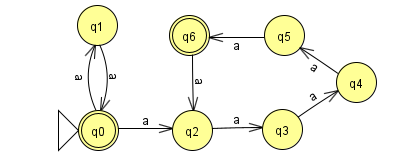
\includegraphics[width=0.5\textwidth]{img/graph6.png}
    \end{center}
    \item The language is regular since there exists an NFA that corresponds to $L_2$. The NFA is shown bellow:
    \begin{center}
        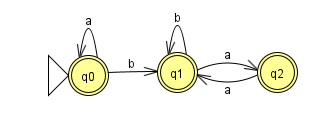
\includegraphics[width=0.5\textwidth]{img/graph7.png}
    \end{center}
    \item The language is regular since there exists an NFA that corresponds to $L_3$. The NFA is shown bellow:
    \begin{center}
        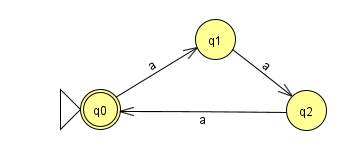
\includegraphics[width=0.5\textwidth]{img/graph8.png}
    \end{center}
    \item
        \begin{proof}
            
        \end{proof}
\end{enumerate}